  
\documentclass[titlepage]{article}
\usepackage[utf8]{inputenc}
\usepackage{amsmath}
\usepackage{tcolorbox}
\usepackage{amssymb}
\usepackage{amsthm}
\usepackage{empheq}
\usepackage{hyperref}
\usepackage{xcolor}
\usepackage{float}
\usepackage{xparse}
\usepackage{mathtools}
\DeclarePairedDelimiter{\ceil}{\lceil}{\rceil}
\usepackage[
top    = 2.50cm,
bottom = 2.50cm,
left   = 2.75cm,
right  = 2.75cm]{geometry}
\usepackage{fancyhdr}
\pagestyle{fancy}
\lhead{AICC 2}
\rhead{EPFL/Alp Ozen}

\newtheorem{remark}{Remark}[section]
\newtheorem{theorem}{Theorem}[section]
\newtheorem{prop}{[Proposition]}
\newtheorem{definition}{Definition}
\newtheorem{question}{Question}

\newcommand{\interior}[1]{%
  {\kern0pt#1}^{\mathrm{o}}%
}
\newcommand{\Rn}{\mathbb{R}^n}
\newcommand{\Rm}{\mathbb{R}^m}
\newcommand{\R}{\mathbb{R}}

\title{\textbf{AICC 2 - Bixio Rimoldi}}
\author{Alp Ozen}
\date{Spring 2019}
\newtheorem{example}{Example}[section]
\newtheorem{axiom}{Axiom}
\newtheorem{cor}{Corollary}

\begin{document}

\maketitle
\tableofcontents
\clearpage

\section{Week 2}

\subsection{Entropy}
We begin by defining \textbf{entropy} as Shannon put it:

\begin{definition}\textbf{Entropy}

Note that this definition assumes base $2$ aka. binary.
$$ H(s) = - \sum_{s \in A} p(s)\log_{2}p(s) \ \text{A being our alpahabet aka. sample space}$$
and thus an equivalent definition is:
$$ H(s) = E[-\log_{2}p(s)]$$
And similarly, Shannon defines information as:
$$-\log_{2}p(s)$$
\end{definition}

For a random distribution we get:

\begin{example}
$$\forall x \in A \ p(x) = \frac{1}{|A|}, \ -\log_{2}p(s) = \log_{2}|A|$$
Hence the entropy function $H(s) = E[\log_{2}|A|]} = \underbrace{\log_{2}|A|}_{\text{do the algebra}}$
\end{example}

And now we present the \textbf{information theory inequality}

\begin{definition}\textbf{IT inequality}
$$ \log_{b}r \leq (r-1)\log_{b}(e)$$
\end{definition}

\begin{proof}
Given that $$\ln(r) \leq (r-1)$$ and that $$ ln(r) = \frac{\log_{b}(r)}{\log_{b}(e)}$$ we are done.
\end{proof}

And now we present the Entropy bound theorem:
\begin{theorem}
$$S \in A \ 0 \leq H(S) \leq \log|A|$$ 
\end{theorem}

\begin{proof}
We only show the RHS as the LHS is more or less trivial. 
Our goal is to show:

\begin{align*}
    \text{need to reach} H(s) - \log|A| \leq 0 \\
    E[-\log p(s)] - \log |A|\\
    = E[\log \frac{1}{p(s)|A|}]\\
    = \sum_{s\in A}p(s)(\log \frac{1}{p(s)|A|})\\
    \leq \underbrace{log(e)\sum[\frac{1}{|A|} - p(s)]}_{\text{using IT ineq.}} = 0
\end{align*}
\end{proof}
\subsection{Source coding}
A code is said to have a prefix if:
\begin{definition}\textbf{Prefix of a code}
\\

For some sequence of characters $a_{1}a_{2}\ldots a_{n}$ and $b_{1}b_{2}\ldots b_{m}$ with $n \leq m$ we have $a_{1}a_{2}\ldots a_{n} =  b_{1}b_{2}\ldots b_{n}$
\end{definition}

A \textbf{prefix free code} also known as \textbf{instantaneouss code} is one that has no prefixes. And now we come to the important \textbf{Kraft-McMillan} result:

\begin{theorem}
If a $D-ary$ code is uniquely decodable, then it satisfies:

$$ D^{-l_{1}} + \ldots + D^{-l_{m}} \leq 1 $$
\textcolor{red}{Note that there are non-instantaneous codes that stil satisfy this inequality. By the same token, by the contrapositive, we have that if a code does not satisfy the inequality, then there exists no prefix-free version of it.}
\end{theorem}

We now define the \textbf{average codeword length}

\begin{definition}\textbf{average codeword length}
$$ L(S,R) = \sum_{s \in A} p_{S}(s)L(R(s)) \ \text{where $L$ represents length}$$
\end{definition}

Given this definition, another important result is:

\begin{theorem} \textbf{Lower bound and Upper bound for average optimal codeword length}
$$H_{d}(S) \leq L(S,R) \leq H_{d}(S) + 1$$
\end{theorem}

This result becomes a useful tool once we realize the similarity in the definitions as below:

\begin{align*}
    H(S) = - \sum p(s)\log p(s)\\
    L(S,R) = \sum p(s)L(R(s))
\end{align*}

Given this, \textit{Shannon - Fano} realized that we may define a code of length $\ceil*{\log_{D} p(s)}$
This satisfies the Kraft inequality hence we now have a method of obtaining uniquely decodable code. 
\\

But as it turns out, Huffman was the first to actually find out how one finds an optimal code. We list our alphabet with probability in increasing order. Then, if say we are working in base 2, we simply continuously combine the smallest probabilities and build our branches from them. Hence, as below, we have that a Huffman code isn't always unique:

\begin{figure}[H]
    \centering
    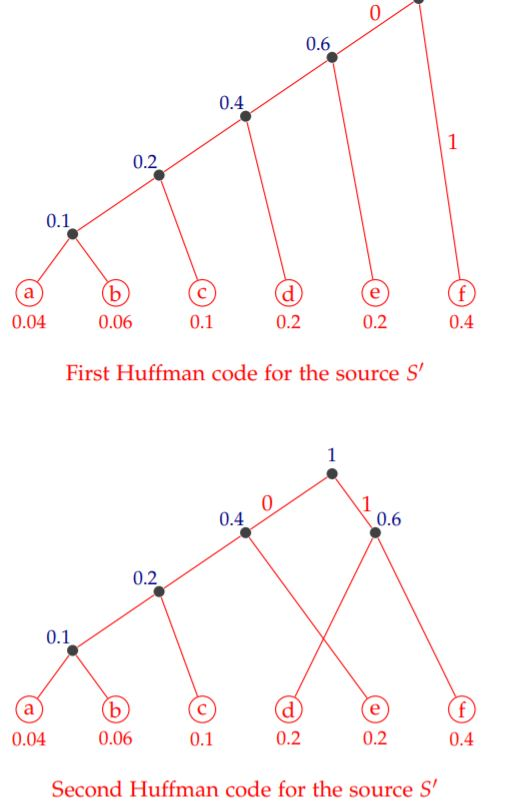
\includegraphics[scale = 0.3]{src/huff.JPG}
    \caption{Huffman codes}
    \label{fig:my_label}
\end{figure}

\section{Week 3}
We now define conditional entropy(the intuition for this being, we want to mesure uncertainty given knowledge of something else) as follows:

\begin{definition}
$$H(X|Y) := - \sum p(x|y)\log p(x|y)$$
\end{definition}

And the law of \textbf{total probability}

\begin{theorem}
Imagine we take a sample space with some subset $A$ and cut it into 3 disjoint units $B_{i}$. Now we may describe the set $A$ as $A = (B_{1} \cap A) \cup (B_{2} \cap A) \cup (B_{3} \cap A)$ This is equivalent to now saying:

$$p(A) = p(B_{1} \cap A) + p(B_{2} \cap A) + p(B_{3} \cap A) $$
Which in terms of conditional probability is $$p(A) = p(A|B_{1})p(B_{1}) + p(A|B_{2})p(B_{2}) + p(A|B_{3})p(B_{3})$$
\end{theorem}

And another useful theorem is:

\begin{theorem}
$$H(s_{1},s_{2},\ldots,s_{n}) \leq H(s_{1}) + H(s_{2}) + \ldots + H(s_{n})$$
with equality iff the $s_{i}$ are independent. 
\end{theorem}

A similar result now is the chain rule of conditional entropy.
\begin{theorem}\textbf{Conditional entropy chain rule}
$$H(S_{1},S_{2},\ldots,S_{n}) = H(S_{1}) + H(S_{2}|S_{1}) + \ldots + H(S_{n}|S_{1},\ldots,S_{n-1})$$
\end{theorem}

To clarify the notation used above, when we write $P_{X_{1}}, \ldots, X_{n}(x_{1},\ldots, x_{n})$ we interpret each comma as an intersection$\cap$

And we now introduce what it means for a source to be \textbf{regular}

\begin{definition}\textbf{Regular source}
\\
A source is regular if
\begin{align*}
    H(S) := \lim_{n\to\infty} H(S_{n})\\
    H^{*}(S) := \lim_{n \to \infty} H(S_{n}|S_{1},S_{2},\ldots,S_{n-1})
\end{align*}

exist and are finite. 
\end{definition}

Now it should be intuitively obvious that conditioning would reduce entropy. Lets prove it.

\begin{theorem}
$$H(X|Y) \leq H(X)$$
\end{theorem}

\begin{proof}
\begin{align*}
    E(\log\frac{1}{p(X|Y)}) + E(\log p(X))\\
    = E(\log\frac{p(X)}{p(X|Y)})\\
    = E(\log\frac{p(X)p(Y)}{p(X|Y)p(Y)})\\
    \leq (\frac{p(X)p(Y)}{p(X\cap Y) - 1}\log(e)
    \leq 0
\end{align*}
\end{proof}

\subsection{Week 4}

We begin by making an important distinction in the definition of conditional entropy.

\begin{definition}\textbf{Conditional entropy given $Y=y$}
\\
We define this as:
$$H(X|Y=y) = - \sum_{x \in (\cdot | y)} P(x|y)\log P(x|y)$$
\end{definition}

Given this definition, the more general definition of conditional entropy is:

\begin{definition}
$$H(X|Y) = - \sum P(y)H(X|Y=y) $$
\end{definition}

And we now introduce a \textbf{stationary source}

\begin{definition}\textbf{Stationary source}
\\
A source is stationary if $\forall n,k$ the blocks $S_{1}, \ldots, S_{n}$ and $S_{n+1}, \ldots, S_{k}$ have the same statistic that is:
\begin{align*}
    P_{s_{1}} = P_{s_{i}}
\end{align*}

\end{definition}


\begin{theorem}
All stationary sources are regular. 
\end{theorem}


\section{Useful links}
Amazing YouTube playlist: \hyperlink{ https://www.youtube.com/playlist?list=PLE125425EC837021F}{YT Information Theory playlist}



\end{document} 
